\documentclass{book}
\usepackage{physics}
\usepackage{graphicx}
\usepackage{caption}
\usepackage{amsmath}
\usepackage{bm}
\usepackage{framed}
\usepackage{authblk}
\usepackage{empheq}
\usepackage{amsfonts}
\usepackage{esint}
\usepackage[makeroom]{cancel}
\usepackage{dsfont}
\usepackage{centernot}
\usepackage{mathtools}
\usepackage{bigints}
\usepackage{amsthm}
\theoremstyle{definition}
\newtheorem{defn}{Definition}[section]
\newtheorem{prop}{Proposition}[section]
\newtheorem{rmk}{Remark}[section]
\newtheorem{thm}{Theorem}[section]
\newtheorem{exmp}{Example}[section]
\newtheorem{prob}{Problem}[section]
\newtheorem{sln}{Solution}[section]
\newtheorem*{prob*}{Problem}
\newtheorem{exer}{Exercise}[section]
\newtheorem*{exer*}{Exercise}
\newtheorem*{sln*}{Solution}
\usepackage{empheq}
\usepackage{tensor}
\usepackage{xcolor}
%\definecolor{colby}{rgb}{0.0, 0.0, 0.5}
\definecolor{MIT}{RGB}{163, 31, 52}
\usepackage[pdftex]{hyperref}
%\hypersetup{colorlinks,urlcolor=colby}
\hypersetup{colorlinks,linkcolor={MIT},citecolor={MIT},urlcolor={MIT}}  



\newcommand*\widefbox[1]{\fbox{\hspace{2em}#1\hspace{2em}}}

\newcommand{\p}{\partial}
\newcommand{\R}{\mathbb{R}}
\newcommand{\C}{\mathbb{C}}
\newcommand{\lag}{\mathcal{L}}
\newcommand{\nn}{\nonumber}
\newcommand{\ham}{\mathcal{H}}
\newcommand{\M}{\mathcal{M}}
\newcommand{\I}{\mathcal{I}}
\newcommand{\K}{\mathcal{K}}
\newcommand{\F}{\mathcal{F}}
\newcommand{\w}{\omega}
\newcommand{\lam}{\lambda}
\newcommand{\al}{\alpha}
\newcommand{\be}{\beta}
\newcommand{\x}{\xi}

\newcommand{\G}{\mathcal{G}}

\newcommand{\f}[2]{\frac{#1}{#2}}

\newcommand{\ift}{\infty}

\newcommand{\lp}{\left(}
\newcommand{\rp}{\right)}

\newcommand{\lb}{\left[}
\newcommand{\rb}{\right]}

\newcommand{\lc}{\left\{}
\newcommand{\rc}{\right\}}


\newcommand{\V}{\mathbf{V}}
\newcommand{\U}{\mathcal{U}}
\newcommand{\Id}{\mathcal{I}}
\newcommand{\D}{\mathcal{D}}
\newcommand{\Z}{\mathcal{Z}}

%\setcounter{chapter}{-1}






\usepackage{subfig}
\usepackage{listings}
\captionsetup[lstlisting]{margin=0cm,format=hang,font=small,format=plain,labelfont={bf,up},textfont={it}}
\renewcommand*{\lstlistingname}{Code \textcolor{violet}{\textsl{Mathematica}}}
\definecolor{gris245}{RGB}{245,245,245}
\definecolor{olive}{RGB}{50,140,50}
\definecolor{brun}{RGB}{175,100,80}

%\hypersetup{colorlinks,urlcolor=colby}
\lstset{
	tabsize=4,
	frame=single,
	language=mathematica,
	basicstyle=\scriptsize\ttfamily,
	keywordstyle=\color{black},
	backgroundcolor=\color{gris245},
	commentstyle=\color{gray},
	showstringspaces=false,
	emph={
		r1,
		r2,
		epsilon,epsilon_,
		Newton,Newton_
	},emphstyle={\color{olive}},
	emph={[2]
		L,
		CouleurCourbe,
		PotentielEffectif,
		IdCourbe,
		Courbe
	},emphstyle={[2]\color{blue}},
	emph={[3]r,r_,n,n_},emphstyle={[3]\color{magenta}}
}


\begin{document}
\begin{titlepage}\centering
 \clearpage
 \title{{\textsc{\textbf{ATOMIC PHYSICS}}}\\ \smallskip - A Quick Guide - \\}
 \author{\bigskip Huan Q. Bui}
  \affil{B.A., COLBY COLLEGE (2021) $\,$\\  
  	MASSACHUSETTS INSTITUTE OF TECHNOLOGY}
 \date{June 15, 2021}
 \maketitle
 \thispagestyle{empty}
\end{titlepage}

\subsection*{Preface}
\addcontentsline{toc}{subsection}{Preface}


$\,$\\


\noindent Greetings, \\


While I have spent most of my undergraduate years in Professor Charles Conover's lab at Colby College working on cold atom experiments, I never had \textit{formal} training in atomic, molecular, and optical physics. The closest to formal training I have for AMO physics is a standard quantum mechanics course I took in the fall of my junior year. Most of the intuition I have for atomic physics, I learned from my discussions with Professor Conover or read from books and articles here and there. This article is my attempt at \textit{formally} teaching myself this subject. It will mostly contain basic/essential concepts in AMO physics. I'll also sprinkle in a few ideas or definitions that are relevant to what I do in Prof. Zwierlein's group. \\

This article is my version of an ``atomic physics dictionary,'' which should keep growing as I go along in my education and research at MIT. As a result, there is no good way for me to organize the topics here but by alphabetical order (hence ``dictionary''). I don't know how well I'll be able to curate this article, but we'll see.\\


In any case, good luck and, most importantly, enjoy!


\newpage





\chapter*{A}

\section*{Avoided crossing}


\begin{figure}[!htb]
	\centering
	\includegraphics*[width=0.75\textwidth]{images/avoided_crossing}
	\caption{From Wikipedia}
\end{figure}


This concept is actually mathematically very easy to describe. Basically, avoided crossing is a phenomenon where two eigenvalues of a Hermitian matrix (say, of a Hamiltonian) which depend on some set of $N$ continuous real parameters cannot become equal (or ``cross'') in value except on a manifold of $N-2$ dimensions. For a mathematically rigorous definition, the reader may refer to the \textcolor{blue}{von Neumann-Wigner theorem}. However, since $N=1$ most of the time, we don't even worry about the second part (``except...'') of the definition.\\


An easy example is two-state systems. Consider a Hamiltonian $\widehat{H} = \text{diag}(E_1, E_2)$ with $E_1$ with off-diagonal perturbation $P$:
\begin{equation*}
\widehat{H}' = \widehat{H} + \widehat{P} = \begin{bmatrix}
E_1 & W \\ W^* & E_2
\end{bmatrix}.
\end{equation*}
Diagonalizing this new Hamiltonian gives the following eigenvalues:
\begin{equation*}
E_{\pm} = \f{1}{2}(E_1 + E_2) \pm \f{1}{2}\sqrt{(E_1 - E_2)^2 + 4\abs{W}^2}
\end{equation*}
Plotting $E_+$ and $E_-$ against $\Delta E = E_1  - E_2$, we get two branches of a parabola. When $W \neq 0$, we see that $E_+ \neq E_-$ when $\Delta  E = 0$. But when $W = 0$, $E_+ = E_-$ at $\Delta E = 0$. We say that the level crossings are avoided due to the perturbation. 


\chapter*{B}


\section*{Bloch's Theorem and Bloch States}


Consider a periodic potential $V(\mathbf{r})$ associated with a lattice whose \textcolor{blue}{primitive lattice translation vectors} are given by 
\begin{equation*}
\mathbf{T} = n_1 \mathbf{a}_1 +  n_2 \mathbf{a}_2  +  n_3 \mathbf{a}_3,
\end{equation*}
where $n_i$ are integers and $\mathbf{a_i}$ are the three noncoplanar vectors ($\mathbf{T}$ is basically vectors which translates from one vertex in the lattice to another arbitrary one). Since $V$ is periodic, we have
\begin{equation*}
V(\mathbf{T} + \mathbf{r}) = V(\mathbf{r}). 
\end{equation*}
In Fourier components, 
\begin{equation*}
V(\mathbf{r}) = \sum_\mathbf{G} V_\mathbf{G} e^{i\mathbf{G}\cdot \mathbf{r}}
\end{equation*}
where $\mathbf{G}$ are a set of vectors and $V_\mathbf{G}$ are Fourier coefficients. By the periodicity of $V$, we have
\begin{equation*}
e^{i\mathbf{G}\cdot \mathbf{T}} = 1 \implies \mathbf{G}\cdot \mathbf{T} = 2\rho \pi, \quad \rho \in \mathbb{Z}.
\end{equation*}
The only way to define $\mathbf{G}$ such that the above equation makes sense is:
\begin{equation*}
\mathbf{G} = m_1 \mathbf{A}_1 + m_2 \mathbf{A}_2 + m_3 \mathbf{A}_3
\end{equation*}
where $m_j$ are integers and $\mathbf{A}_j$ are three noncoplanar vectors defined by 
\begin{equation*}
\mathbf{a}_j \cdot \mathbf{A}_l = 2\pi \delta_{jl}
\end{equation*}
This shows the existence of an $r$-lattice implies that of a $k$-lattice, and we call $\mathbf{G}$ the \textcolor{blue}{reciprocal lattice}. \\


What set of functions describes the motion of electrons in such a potential? Since we want to reflect the translation symmetry of the lattice, we may impose the \textit{Born-von Karman periodic boundary condition} on the plane wave 
\begin{equation*}
\phi(\mathbf{r}) = e^{i(\mathbf{k}\cdot \mathbf{r} - \omega t)}
\end{equation*}
to get
\begin{equation*}
\phi(\mathbf{r} + N_j \mathbf{a_j}) = \phi(\mathbf{r})
\end{equation*}
where $j=1,2,3$ and $N = N_1N_2N_3$ is the number of primitive unit cells in the crystal; $N_j$ is the number of unit cells in the $j$th direction. From here, we have that 
\begin{equation*}
e^{iN_j \mathbf{k}\cdot \mathbf{a}_j} = 1.
\end{equation*}
Following a similar argument as before, we find that the only allowed $\mathbf{k}$ vectors are of the form
\begin{equation*}
\mathbf{k} = \sum^3_{j=1}\f{m_j}{N_j}\mathbf{A}_j
\end{equation*}








Now, consider a Schr\"{o}dinger equation with potential $V(\mathbf{r})$:
\begin{equation*}
\widehat{H}\psi = \lb -\f{\hbar^2 \nabla^2}{2m} + V(\mathbf{r}) \rb \psi = E\psi.
\end{equation*}
In Fourier components, we again have
\begin{equation*}
V(\mathbf{r}) = \sum_\mathbf{G} V_\mathbf{G} e^{i\mathbf{G}\cdot \mathbf{r}}.
\end{equation*}
Let us set the background potential to zero, i.e., $V_0 \equiv 0$. Next, let us write the solution $\phi(\mathbf{r})$ as a combination of plane waves obeying the Born-von Karman PBC:
\begin{equation*}
\psi(\mathbf{r}) = \sum_\mathbf{k}C_\mathbf{k} e^{i\mathbf{k}\cdot \mathbf{r}},
\end{equation*}
so that $\phi(\mathbf{r})$ also satisfies the Born-von Karman PBC. Plugging this into the SE, we find 
\begin{equation*}
\sum_\mathbf{k} \f{\hbar^2k^2}{2m} C_\mathbf{k} e^{i\mathbf{k}\cdot \mathbf{r}} + \underbrace{\lb \sum_\mathbf{G} V_\mathbf{G} e^{i\mathbf{G}\cdot \mathbf{r}} \rb \lb \sum_\mathbf{k} C_\mathbf{k} e^{i\mathbf{k}\cdot \mathbf{r}} \rb}_{V(\mathbf{r}\psi)} = E\sum_\mathbf{k} C_\mathbf{k} e^{i\mathbf{k}\cdot \mathbf{r}}
\end{equation*}
where we can re-write:
\begin{equation*}
V(\mathbf{r})\psi = \sum_{\mathbf{G},\mathbf{k}} V_\mathbf{G}C_\mathbf{k} e^{i(\mathbf{G}+ \mathbf{k})\cdot \mathbf{r}}  = \sum_{\mathbf{G},\mathbf{k}} V_\mathbf{G}C_{\mathbf{k}-\mathbf{G}} e^{i\mathbf{k}\cdot \mathbf{r}}.
\end{equation*}
With this, we can factor out $e^{i\mathbf{k}\cdot \mathbf{r}}$ in each term of the SE and use the fact that the plane waves form an orthogonal basis, we find 
\begin{equation*}
\lp \f{\hbar^2k^2}{2m} - E \rp C_\mathbf{k} + \sum_\mathbf{G} V_\mathbf{G} C_{\mathbf{k}-\mathbf{G}} = 0.
\end{equation*}

Let us write $\mathbf{k} = \mathbf{q} - \mathbf{G}'$ and let $\mathbf{G}'' = \mathbf{G}' + \mathbf{G}$, where $\mathbf{q}$ lies in the \textcolor{blue}{first Brillouin zone}. With this change of variables, we have the result
\begin{equation*}
\lp \f{\hbar^2 (\mathbf{q} - \mathbf{G}')^2}{2m} - E \rp C_{\mathbf{q} - \mathbf{G}'} + \sum_{\mathbf{G}''}V_{\mathbf{G}'' - \mathbf{G}'}C_{\mathbf{q} - \mathbf{G}''} = 0.
\end{equation*}


Now, we're ready for the statement of the \textbf{Bloch's Theorem}. The result above involves coefficients $C_{\mathbf{k}}$ in which $\mathbf{k} = \mathbf{q} - \mathbf{G}$, where $\mathbf{G}$ are general reciprocal lattice vectors. This means that if we fix $\mathbf{q}$, then the only $C_\mathbf{k}$ that feature are of the form $C_{\mathbf{q} - \mathbf{G}}$. In other words, for each $\mathbf{q}$, there is a wavefunction $\psi_\mathbf{q}(r)$ that takes the form
\begin{equation*}
\psi_\mathbf{q}(\mathbf{r}) = \sum_\mathbf{G} C_{\mathbf{q} - \mathbf{G}} e^{i(\mathbf{q} - \mathbf{G})\cdot \mathbf{r}},
\end{equation*}
where we have substituted $\mathbf{k} = \mathbf{q} - \mathbf{G}$. Factoring out $e^{i\mathbf{q}\cdot \mathbf{r}}$, we find 
\begin{equation*}
\boxed{\psi_\mathbf{q}(\mathbf{r})  = e^{i\mathbf{q}\cdot \mathbf{r}} \sum_\mathbf{G} C_{\mathbf{q} - \mathbf{G}} e^{-i \mathbf{G}\cdot \mathbf{r}} \equiv e^{i\mathbf{q}\cdot\mathbf{r}}u_{j,\mathbf{q}}}
\end{equation*}
So, the solution is a plane wave with wave vector within the first Brillouin zone TIMES a function with the periodicity of the lattice. Functions of this form are known as \textbf{Bloch functions} or \textbf{Bloch states}. They serve as a suitable basis for the wave functions or states of electrons in crystalline solids. \\



\textbf{Bloch's Theorem} is as follows: \textit{The eigenstates $\psi$ of a one-electron Hamiltonian defined above for all Bravais lattice translation vectors $\mathbf{T}$ can be chosen to be a plane wave times a function with the periodicity of the Bravais lattice.} We note two things:
\begin{itemize}
	\item This is true for any particle propagating in a lattice
	\item The theorem makes no assumption about the \textit{strength/depth} of the potential. 
\end{itemize}









\hrule 


\noindent \textbf{Notes:} The terminologies in \textcolor{blue}{blue} can be found in \cite{kittel1996introduction} or Wikipedia. The concepts are simple enough, so I won't include their definitions here. 














\section*{Bose-Einstein Condensate (BEC)}









%%%%%%%%%%%%%%%%%%%%%%%%%%%%%%%%%%%%%%%
\chapter*{C}
%%%%%%%%%%%%%%%%%%%%%%%%%%%%%%%%%%%%%%%
\chapter*{D}



\section*{Doppler temperature}


Doppler temperature is the minimum temperature achievable with Doppler cooling. When an atom absorbs a counter-propagating photon, its velocity decreases due to momentum conservation. The atom then re-emits the photon (via spontaneous emission) in a random direction, giving the atom a momentum kick in a random direction. The random kicks average to zero, so the atom averages a zero mean velocity, i.e., $< v > = 0$. However, $<v^2> \neq 0$, so there is heat supplies to the atom. At equilibrium, the heating and cooling rates are equal; this is the limit on the amount by which the atom can be cooled using this technique. \\

If the transitions used for Doppler cooling have natural linewidths $\gamma$, then the Doppler temperature is given by 
\begin{equation*}
T_\text{Doppler} = \f{\hbar \gamma}{2k_B}
\end{equation*} 
where $k_B$ is the Boltzmann constant. This is usually much higher than the \textcolor{blue}{recoil temperature}, which is the temperature associated with the momentum gained from spontaneous emission. 
%%%%%%%%%%%%%%%%%%%%%%%%%%%%%%%%%%%%%%%
\chapter*{E}
%%%%%%%%%%%%%%%%%%%%%%%%%%%%%%%%%%%%%%%
\chapter*{F}


\section*{Feshbach Resonance (in ultracold gases)}


To start, let us look at some results in scattering theory. For more information about this topic, the reader may refer to \cite{sakurai1995modern}. Consider a general wave-scattering problem where we have an incident plane wave with wave number $k$ and a radial scattered wave with anisotropy term (partial wve scattering amplitude) $f(\theta)$: 
\begin{equation*}
\phi_\text{inc} = e^{ikz}, \quad \phi_{\text{sc}} = \f{f(\theta)e^{ikr}}{r}
\end{equation*}
and by definition
\begin{equation*}
d\sigma = \abs{f(\theta)}^2\, d\Omega.
\end{equation*}
Consider a particle of mass $m$, energy $\hbar^2k^2/2m$, in a central potential $V(r)$. At large $r$, the wave function is approximated by the sum of the waves above:
\begin{equation*}
\phi_{\text{large } r} = \phi_{\text{inc}} + \phi_{\text{sc}}. 
\end{equation*}
Since $\phi_{\text{large } r}$ must also solve the SE, which is separable due to $V(r)$ being central, we have \cite{bohm2012quantum}
\begin{equation*}
\phi_{\text{large } r} = Y(\theta)R(r) = \lp \sum^\infty_{l=0} C_l P_l(\cos\theta) \rp \f{1}{kr}\sin\lp kr - \f{l\pi}{2} + \delta_l \rp
\end{equation*}
By re-writing $\phi_\text{large $r$}$ like this we find 
\begin{equation*}
f(\theta) = \f{1}{k}\sum^\infty_{l=0} \sin \delta_l P_l(\cos\theta).
\end{equation*}
Here $l$, the angular momentum quantum number, corresponds to different partial waves. \\

Now recall the radial SE:
\begin{equation*}
-\f{\hbar^2}{2m}\f{d^2 u(r)}{dr^2} + V_\text{eff}(r)u(r) = Eu(r)
\end{equation*} 
where
\begin{equation*}
V_\text{eff}(r) = V(r) + \f{\hbar^2l(l+1)}{2mr^2}.
\end{equation*}
The form of $V_\text{eff}$ implies that the particles cannot reach small $r$'s for $l>0$. So, by assuming that $V(r)$ is only significant/nontrivial for small $r$, we find that only $l=0$ matters. So, we only care about $s$-waves in the expansion. With this, we have
\begin{equation*}
\phi_{\text{large } r} = \f{C_0}{kr} \sin(kr - \delta_0) = 
\end{equation*}
This means that
\begin{equation*}
f = -\f{1}{k}e^{i\delta_0 }\sin\delta_0 = \f{1}{k\cot\delta_0 -ik}. 
\end{equation*}

The \textcolor{blue}{$s$-wave scattering length} $a$ is defined as 
\begin{equation*}
a = -\lim_{k\to 0}\f{\tan \delta_0 (k)}{k}
\end{equation*}
\begin{itemize}
	\item For strong and attractive interactions, $a$ is large and negative
	
	\item For strong and repulsive interactions, $a$ is large and positive. 
\end{itemize}
By Taylor expansion we have
\begin{equation*}
k\cos(\delta_0(k)) \approx -\f{1}{a} + \f{1}{2}r_\text{eff} k^2 + \dots
\end{equation*}
where $r_\text{eff}$ is the effective range of the potential. Plugging this back into the equation for $f$ we find 
\begin{equation*}
f(k) = \f{1}{-1/a + r_\text{eff} k^2/2 - ik}.
\end{equation*}
From the Lippmann-Schwinger equation for $s$-waves, we find that 
\begin{equation*}
\f{1}{f(k)} \approx -\f{4\pi}{v_0} + \f{4\pi}{v_0} \int\f{d^3q}{(2\pi)^3} \f{v(\mathbf{q})}{k^2 - q^2 - i\eta}
\end{equation*}
where $v(\cdot)$ is the interatomic potential. 







\section*{Free spectral range (FSR)}


%%%%%%%%%%%%%%%%%%%%%%%%%%%%%%%%%%%%%%%
\chapter*{G}
%%%%%%%%%%%%%%%%%%%%%%%%%%%%%%%%%%%%%%%
\chapter*{H}
%%%%%%%%%%%%%%%%%%%%%%%%%%%%%%%%%%%%%%%
\chapter*{I}
%%%%%%%%%%%%%%%%%%%%%%%%%%%%%%%%%%%%%%%
\chapter*{K}
%%%%%%%%%%%%%%%%%%%%%%%%%%%%%%%%%%%%%%%
\chapter*{L}
%%%%%%%%%%%%%%%%%%%%%%%%%%%%%%%%%%%%%%%
\chapter*{M}



\section*{Magnetic evaporative cooling}






\section*{Magneto-optical trap (MOT)}

The idea of a MOT is actually quite intuitive. However, there are subtle details that one needs to know in order to truly understand its principle of operation. 

\begin{figure}[!htb]
	\centering
	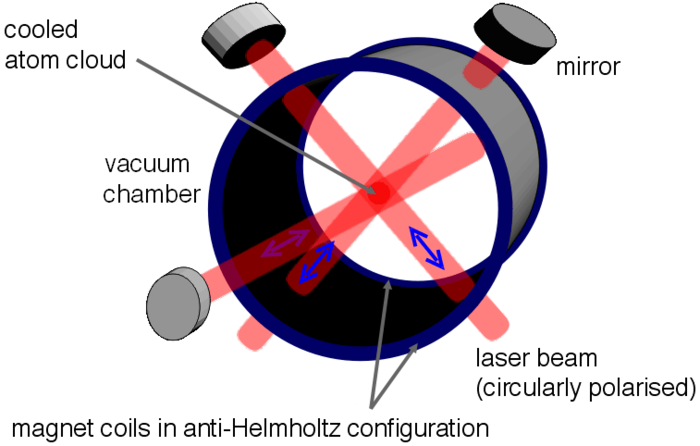
\includegraphics[width=0.75\textwidth]{images/MOT}
	\caption{From Wikipedia}
\end{figure}

Magneto-optical traps use a combination of red-detuned, circularly polarized, counter-propagating lasers, and a quadrupole magnetic field to trap neutral atoms with admissible atomic structure (i.e. not all atomic species can be magneto-optically trapped). \\


A theoretical description of a MOT is as follows. First, we require a vacuum and two coils in an anti-Helmholtz configuration. We let the coils be separated along the $z$-axis. To first order approximation (i.e. near the center), the magnetic field takes the form
\begin{equation*}
\vec{B} = B_0 \lp \f{x}{2}, \f{y}{2}, -z \rp, \quad B_0 = -\f{3\mu_0 I a R^2}{2(R^2 + a^2)^{5/2}}
\end{equation*}
where $R$ is the (common) radius of the coils and $2a$ is the distance between two coils. From here, we see that field strength is linear in position, and that the field gradient is twice as strong along the $z$ direction than along $x$ or $y$. 


\begin{figure}[!htb]
	\centering
	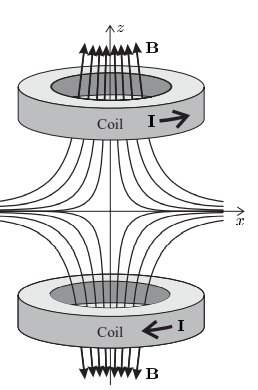
\includegraphics[width=0.4\textwidth]{images/anti-helmholtz}
	\caption{From \cite{foot2005atomic}.}
\end{figure}

Consider an atom with ground and excited states with $J=0$ and $J=1$, respectively. The Zeeman effect due to the magnetic field lifts the degeneracy in the $m_J$'s. For $J=1$ there are now $2J+1 = 3$ nondegenerate sublevels. For $J=0$ there is no such splitting. Since the magnetic field varies in space, the Zeeman effect on the atoms also varies in space, being more extreme for atoms further away from the center of the trap. \\


Next, we add three pairs of counter-propagating circularly-polarized orthogonal laser beams. The lasers are red-detuned from the $J=0 \to J=1$ transition. Circular polarization is required because we only want to selectively drive transitions from $\ket{0,0}$ to a specific $\ket{1,m_J}$ depending on where the atom is in the magnetic field. \\


When the atoms are the center of the trap, they don't experience any Zeeman shift and don't see the red-detuned light (not very much). They are the coldest and darkest atoms.\\


For an atom moving in the $+z \neq 0$ direction, for instance, the Zeeman effect shifts the energy of $\ket{J=1,m_J=-1}$ down closer to the energy of $\ket{J=0,m_J=0}$. In the $z$ direction, there are also the counter-propagating $\sigma^-$ and $\sigma^+$ in the $- z$ and $+z$ directions, respectively. Due to the Doppler effect, the atom moving in the $+z$ direction gets closer to resonance with the $\sigma^-$ beam traveling in the $-z$ direction, which drives the $\Delta m_J = -1$ transition, and feels a stronger scattering force the further it moves away from the center. When the atom absorbs a $\sigma^-$ photon, it goes to the $\ket{J=1,m_J=-1}$ state and gets a momentum kick opposite to its motion. It will eventually re-emits the photon due to spontaneous emission, but since the process is random and averages out to zero we see the atom affected mostly by the absorption of the $\sigma^-$ photon. The net effect is that the atom is pushed towards the center of the trap. Similarly, the atom moving the $-z$ direction is also pushed towards the center. The same thing happens in the $x-$ and $y-$directions.  
 	
 	
\begin{figure}[!htb]
	\centering
	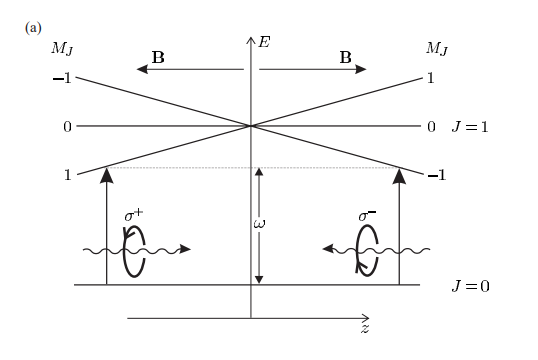
\includegraphics[width=0.75\textwidth]{images/foot_1}
	\caption{From \cite{foot2005atomic}}
\end{figure}

\begin{figure}[!htb]
	\centering
	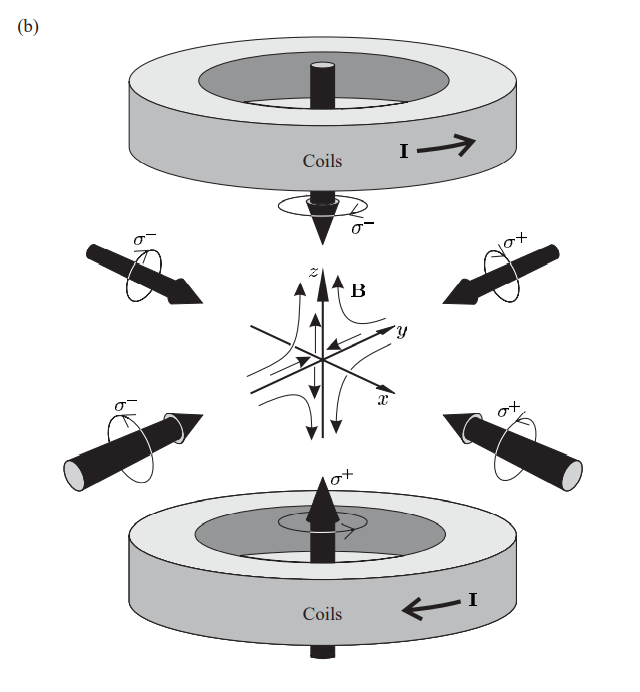
\includegraphics[width=0.7\textwidth]{images/foot_2}
	\caption{From \cite{foot2005atomic}}
\end{figure}


%%%%%%%%%%%%%%%%%%%%%%%%%%%%%%%%%%%%%%%
\chapter*{N}
%%%%%%%%%%%%%%%%%%%%%%%%%%%%%%%%%%%%%%%
\chapter*{O}



\section*{Optical lattice}


\section*{Optical dipole trap}


\section{Optical tweezer}


%%%%%%%%%%%%%%%%%%%%%%%%%%%%%%%%%%%%%%%
\chapter*{P}



\section*{Perturbation theory in QM (simple version)}





\section*{Pound-Drever-Hall (PDH) technique}
%%%%%%%%%%%%%%%%%%%%%%%%%%%%%%%%%%%%%%%
\chapter*{Q}

\section*{Quantum Harmonic Oscillator}

This is one of the most important concepts in quantum mechanics that is applied almost all the time in AMO physics, so it is \textit{very} good to know. \\


In one dimension, the Hamiltonian is given by 
\begin{equation*}
\widehat{H} = \f{\widehat{p}^2}{2m} + \f{1}{2}k\widehat{x}^2 =  \f{\hat{p}^2}{2m} + \f{1}{2}m\omega^2 \widehat{x}^2,
\end{equation*}
where $m$ is the particle mass, $\omega = \sqrt{k/m}$ is the angular frequency of the particle, and $\widehat{x}$ and $\widehat{p}$ are the position and momentum operators, respectively. The wavefunction of the particle satisfies the time-independent SE says $\widehat{H}\ket{\psi} = E\ket{\psi}$. In position space, the solution space for $\widehat{H}$ is spanned by the following Hermite functions
\begin{equation*}
\bra{x}\ket{\psi} = \psi_n = \f{1}{\sqrt{2^n n!}} \lp \f{m\omega}{\pi \hbar} \rp^{1/4} e^{-m\omega^2 x/2\hbar} H_n\lp \f{\sqrt{m\omega}}{\hbar} x \rp
\end{equation*}
where $n \in \mathbb{N}$ and $H_n$ are Hermite polynomials. The corresponding energy levels are 
\begin{equation*}
E_n = \hbar \omega \lp n + \f{1}{2} \rp,
\end{equation*}
and so the zero-point energy is $\hbar\omega/2$, which is non-zero due to the Heisenberg uncertainty principle. We notice that the energies are quantized and adjacent levels are equally spaced by one unit of $\hbar\omega$. We note also that when the \textcolor{blue}{harmonicity} of the potential is lost, we are no longer guaranteed equal spacings between adjacent levels. \\


One way to solve the QHO problem is by using ladder operators (so that we avoid Hermite functions, etc.). We define the creation and annihilation operators as below:
\begin{equation*}
\widehat{a}^\dagger = \sqrt{\f{m\omega}{2\hbar}} \lp \widehat{x} - \f{i}{m\omega}\widehat{p} \rp, \quad \widehat{a} = \sqrt{\f{m\omega}{2\hbar}} \lp \widehat{x} + \f{i}{m\omega}\widehat{p} \rp
\end{equation*}
from which we can represent the position and momentum operators as 
\begin{equation*}
\widehat{x} = \sqrt{\f{\hbar}{2m\omega}} (\widehat{a}^\dagger + \widehat{a}), \quad \widehat{p} = i\sqrt{\f{\hbar m\omega}{2}}(\widehat{a}^\dagger - \widehat{a}).
\end{equation*}
Creation and annhilation operators are not Hermitian. Rather, they are idempotents. They act on the energy eigenstates the following way:
\begin{equation*}
\widehat{a}\ket{n} = \sqrt{n}\ket{n-1}, \quad a\ket{0} = 0, \quad \widehat{a}^\dagger\ket{n} = \sqrt{n+1}\ket{n+1}.
\end{equation*}
This explains why these operators are called the way they are. The number operator $\widehat{N}$ can be defined from the ladder operators:
\begin{equation*}
\widehat{N}\ket{n} \equiv \widehat{a}^\dagger \widehat{a}\ket{n} = n\ket{n}, 
\end{equation*}
and so 
\begin{equation*}
\widehat{H} = \hbar\omega\lp \widehat{a}^\dagger \widehat{a} + \f{1}{2} \rp = \hbar\omega \lp \widehat{N} + \f{1}{2} \rp.
\end{equation*}
With these definitions, one can express any excited state in terms of the ground state:
\begin{equation*}
\ket{n} = \f{(\widehat{a}^\dagger)^n}{\sqrt{n!}} \ket{0}.
\end{equation*}
The QHO can be easily generalized to an $N$-dimensional isotropic QHO by simply repeating the 1D problem $N$ times. The energy is given by 
\begin{equation*}
E = \hbar\omega\lp n_1 + n_2 + \dots + n_N + \f{N}{2} \rp.
\end{equation*}



%%%%%%%%%%%%%%%%%%%%%%%%%%%%%%%%%%%%%%%
\chapter*{R}


\section*{Raman cooling}


\section*{Raman side-band cooling}

Raman side-band cooling is a sub-technique of Raman cooling. This cooling technique starts from atoms in a MOT, with an optical lattice present. We assume that the optical lattice is sufficiently deep that each site is essentially a harmonic trap. Since the atoms are not in the their ground state, they will be trapped in one of the excited levels of the quantum harmonic oscillator. Raman side-band cooling aims to bring these atoms to the ground state of the harmonic potential at each site, and it requires access to the atomic structure of the atoms. \\


Suppose the atom has two levels with ground state $F=1$, such that there is a three-fold degeneracy $m_F = -1,0,1$. A magnetic field is added to induce Zeeman shifts, lifting the degeneracy. The magnetic field strength is tuned such that the Zeeman splitting between the $\Delta m_F = 1$ states matches the spacing of the two levels in the harmonic potential.


\begin{figure}[!htb]
	\centering
	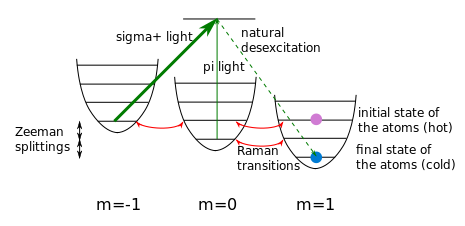
\includegraphics[width=0.75\textwidth]{images/raman_sideband}
	\caption{From Wikipedia}
\end{figure}


By Raman processes, one can transfer an atom to a state whose $m_F$ and vibrational state has changed by $-1$. After all this, the atoms in the lowest vibrational state of the harmonic trap, except for those with $m_F = 1$, are optically pumped to the $m_F = 1$ state using $\sigma_+$ and $\pi$ light. 






\section*{Recoil temperature}

Consider an atom undergoing spontaneous emission of a single photon whose momentum is $p = \hbar k$. By momentum conservation, the momentum kick that the atom gains is also $p$, and its kinetic energy is $p^2/2m = \hbar^2k^2/2m$. The recoil temperature is given by 
\begin{equation*}
T_r = \f{\hbar^2k^2}{k_Bm}.
\end{equation*} 
There is a factor of $1/2$ in an alternative definition, which can be obtained from setting $T_r k_B = p^2/2m$. But I'm following the convention set by \cite{metcalf2007laser}, which does not include the factor of $1/2$.



%%%%%%%%%%%%%%%%%%%%%%%%%%%%%%%%%%%%%%%
\chapter*{S}


\section*{Stark effect}

\section*{Sisyphus cooling}


%%%%%%%%%%%%%%%%%%%%%%%%%%%%%%%%%%%%%%%
\chapter*{T}
%%%%%%%%%%%%%%%%%%%%%%%%%%%%%%%%%%%%%%%
\chapter*{U}
%%%%%%%%%%%%%%%%%%%%%%%%%%%%%%%%%%%%%%%
\chapter*{V}
%%%%%%%%%%%%%%%%%%%%%%%%%%%%%%%%%%%%%%%
\chapter*{W}
%%%%%%%%%%%%%%%%%%%%%%%%%%%%%%%%%%%%%%%
\chapter*{X}
%%%%%%%%%%%%%%%%%%%%%%%%%%%%%%%%%%%%%%%
\chapter*{Y}
%%%%%%%%%%%%%%%%%%%%%%%%%%%%%%%%%%%%%%%
\chapter*{Z}



\section*{Zeeman slower}
%%%%%%%%%%%%%%%%%%%%%%%%%%%%%%%%%%%%%%%



\newpage

\bibliography{Bui_AMO} 
\bibliographystyle{ieeetr}


\end{document}